\section{Lý thuyết Double Machine Learning cho SSI}

\subsection{Mô hình bài toán}

Mô hình cơ bản của bài báo là:
\[
    Y_t = \theta_0\, D_t + g_0(X_t) + \varepsilon_t
\]

Trong đó:
\begin{itemize}
    \item \(\theta_0\): \textbf{tác động điều trị (treatment effect)} cần ước lượng. Ký hiệu \(_0\) chỉ \textit{giá trị thực ở tổng thể (true value)}.
    \item \(g_0(X_t)\): \textbf{hàm nhiễu (nuisance function)} --- kỳ vọng điều kiện của các yếu tố gây nhiễu lên kết quả; phi tuyến và không biết trước.
    \item \(\varepsilon_t\): nhiễu ngẫu nhiên.
\end{itemize}

Mục tiêu duy nhất là ước lượng \(\theta_0\) một cách \textbf{không chệch}, dù \(g_0\) phức tạp và phải học bằng máy. Khi có trạng thái chung \(H_t\), mô hình mở rộng thành:
\[
    Y_t = \theta_0\, D_t + g_0(X_t, H_t) + \varepsilon_t
\]

\subsection{Ý tưởng cốt lõi: Định lý Frisch-Waugh-Lovell (FWL)}

DML tìm tác động điều trị dựa trên ý tưởng từ \textbf{Định lý Frisch-Waugh-Lovell}: trong hồi quy tuyến tính, \(\theta_0\) có thể được cô lập bằng cách làm sạch ảnh hưởng của \(X\) khỏi cả \(Y\) lẫn \(D\).

\textbf{Bước 1 --- Làm sạch \(Y\):}
\begin{enumerate}
    \item Hồi quy \(Y\) theo \(X\) để thu được dự đoán \(\hat{l}(X_t, H_t) \approx \mathbb{E}[Y \mid X, H]\)
    \item Tính phần dư: \(\tilde{Y}_t = Y_t - \hat{l}(X_t, H_t)\)
\end{enumerate}

\textbf{Bước 2 --- Làm sạch \(D\):}
\begin{enumerate}
    \item Hồi quy \(D\) theo \(X\) để thu được propensity score \(\hat{m}(X_t) \approx \mathbb{E}[D \mid X]\)
    \item Tính phần dư: \(\tilde{D}_t = D_t - \hat{m}(X_t)\)
\end{enumerate}

\textbf{Bước 3 --- Hồi quy phần dư:} Hồi quy \(\tilde{Y}\) theo \(\tilde{D}\):
\[
    \tilde{Y}_t = \theta_0\, \tilde{D}_t + u_t \implies \hat{\theta} \xrightarrow{p} \theta_0
\]

DML (Chernozhukov et al., 2018) tổng quát hóa ý tưởng này: thay vì dùng hồi quy tuyến tính để làm sạch, sử dụng các mô hình học máy linh hoạt.

\subsection{Vấn đề khi Cross-Fitting gặp SSI}

Trong DML thông thường, \textbf{cross-fitting (K-fold)} được dùng để tránh overfitting: học mô hình trên các fold train, tính phần dư trên fold test còn lại. Tuy nhiên, khi có trạng thái chung \(H_t\), cross-fitting không còn hợp lệ vì hai lý do:

\paragraph{Vấn đề 1 --- Data Leakage qua \(H_t\):}
\(H_t\) được tính từ \(W_{t-1} = (D_{t-1}, Y_{t-1}, H_{t-1})\) --- toàn bộ thông tin của bước liền trước. Khi bước \(t\) thuộc fold test nhưng bước \(t-1\) thuộc fold train, bộ ước lượng \(\hat{l}, \hat{m}\) đã gián tiếp ``thấy'' quan sát test thông qua \(H_t\). Phần dư \(\tilde{Y}_t\) bị thu hẹp giả tạo (overfit), kéo \(\hat{\theta}\) về phía 0 --- \textbf{ước lượng bị chệch}.

\paragraph{Vấn đề 2 --- Lệch phương sai ước lượng:}
\(H_t\) tạo \textbf{tương quan chuỗi} giữa các hàm score \(\phi_t\), khiến công thức phương sai DML thông thường (chỉ tính phần tổng phương sai, bỏ qua hiệp phương sai) trở nên sai lệch:
\[
    \operatorname{Var}(\hat{\theta}) = \frac{1}{T}\sum_t \operatorname{Var}(\phi_t) + \frac{2}{T}\sum_{t < s} \operatorname{Cov}(\phi_t, \phi_s)
\]
Bỏ qua phần \(\operatorname{Cov}\) làm khoảng tin cậy và \(p\)-value \textbf{không còn hiệu lực}.

\begin{figure}[H]
    \centering
    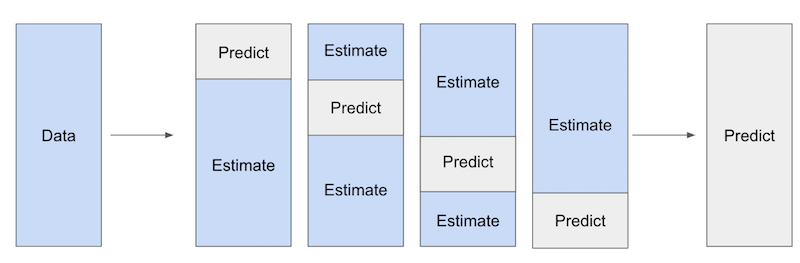
\includegraphics[width=0.78\textwidth]{image/cross-prediction.png}
    \caption{Minh họa cross-fitting K-fold: mỗi fold lần lượt được giữ lại để \textbf{Predict} (test); các fold còn lại dùng để \textbf{Estimate} (học \(\hat{l}, \hat{m}\)). Phần dư out-of-fold không bị overfit vì mô hình chưa từng thấy quan sát đó.}
    \label{fig:cross-fitting}
\end{figure}

\subsection{Giải pháp 1: Auxiliary Data (Dữ liệu phụ trợ độc lập)}

Thay vì cross-fitting, bài báo đề xuất dùng một tập dữ liệu phụ trợ \(W_{\text{aux}}\) \textbf{độc lập} với tập suy luận \(W_{1:T}\):

\begin{algorithm}[H]
\caption{Double Machine Learning for Shared-State Interference (DML4SSI)}
\begin{algorithmic}[1]
    \State \textbf{Bước 1:} Học nuisance functions \(\hat{\eta} = (\hat{l}, \hat{m})\) từ \(W_{\text{aux}}\)
    \State \textbf{Bước 2:} Áp \(\hat{l}, \hat{m}\) lên \(W_{1:T}\) để tính phần dư \(\tilde{Y}_t, \tilde{D}_t\)
    \State \textbf{Bước 3:} Tính \(\hat{\psi} \stackrel{\text{def}}{=} \psi(W_{1:T}, \hat{\eta})\) --- hồi quy phần dư
    \State \Return \(\hat{\psi}\)
\end{algorithmic}
\end{algorithm}

Vì \(W_{\text{aux}} \perp W_{1:T}\), phần dư \(\tilde{Y}, \tilde{D}\) không bị overfit, đảm bảo \(\hat{\theta}\) tiệm cận không lệch dù \(H_t\) phụ thuộc theo thời gian.

\begin{figure}[H]
\centering
\begin{tikzpicture}[
    font=\small,
    box/.style={draw, rounded corners=5pt, thick, minimum height=1.6cm,
                text width=#1, align=center, inner sep=6pt},
    arr/.style={->, >=stealth, thick},
    perp/.style={draw, dashed, green!60!black, rounded corners=5pt, thick,
                 inner sep=6pt, fill=green!6},
]

% ── Top row ──────────────────────────────────────────────────
\node[box=2.0cm, fill=blue!15, draw=blue!60] (Waux) at (0,0) {
    \textbf{Tập phụ trợ}\\[2pt]
    $W_{\text{aux}}$\\[2pt]
    {\footnotesize\itshape độc lập với $W_{1:T}$}
};

\node[box=4.2cm, fill=gray!15, draw=gray!50, right=1.0cm of Waux] (step1) {
    \textbf{Bước 1 · Train nuisance $\hat{\eta}$}\\[4pt]
    \begin{tabular}{cc}
        \colorbox{blue!25}{$\hat{l}(X_t,H_t)$} & \colorbox{violet!20}{$\hat{m}(X_t,H_t)$} \\[2pt]
        {\tiny outcome model} & {\tiny propensity model}
    \end{tabular}
};

\node[perp, right=0.8cm of step1, minimum height=1.6cm, text width=2.2cm, align=center] (badge) {
    {\small $W_{\text{aux}} \perp W_{1:T}$}\\[3pt]
    {\footnotesize $\hat{\eta}$ không thấy $W_{1:T}$}\\
    {\footnotesize $\Rightarrow$ phần dư không overfit}
};

\draw[arr, blue!60] (Waux) -- node[above,font=\scriptsize]{train} (step1);

% ── Down arrow ───────────────────────────────────────────────
\node[below=0.5cm of step1, font=\scriptsize, blue!70] (lbl) {apply $\hat{\eta}$ lên $W_{1:T}$};
\draw[arr, blue!70] (step1.south) -- (lbl.north);

% ── Bottom row ───────────────────────────────────────────────
\node[box=2.0cm, fill=orange!15, draw=orange!60, below=0.9cm of Waux] (W1T) {
    \textbf{Tập chính}\\[2pt]
    $W_{1:T}$\\[2pt]
    {\footnotesize\itshape chuỗi Markov}
};

\node[box=4.2cm, fill=yellow!20, draw=yellow!60!black, right=1.0cm of W1T] (step2) {
    \textbf{Bước 2 · Tính phần dư}\\[4pt]
    $\tilde{Y}_t = Y_t - \hat{l}(X_t,H_t)$\\[2pt]
    $\tilde{D}_t = D_t - \hat{m}(X_t,H_t)$
};

\node[box=2.2cm, fill=green!15, draw=green!60!black, right=1.0cm of step2] (step3) {
    \textbf{Bước 3}\\[2pt]
    $\tilde{Y}_t = \hat{\theta}\,\tilde{D}_t + u_t$\\[4pt]
    $\hat{\theta} \xrightarrow{p} \theta_0$
};

\draw[arr, orange!70] (W1T) -- (step2);
\draw[arr, yellow!60!black] (step2) -- (step3);
\draw[arr, blue!70] (lbl.south) -- (step2.north);

\end{tikzpicture}
\caption{Pipeline Auxiliary Data cho DML4SSI. Vì \(\hat{l}, \hat{m}\) được học từ \(W_{\text{aux}} \perp W_{1:T}\), phần dư \(\tilde{Y}, \tilde{D}\) không bị overfit và \(\hat{\theta}\) tiệm cận không lệch.}
\label{fig:aux-pipeline}
\end{figure}

\subsection{Giải pháp 2: Block Cross-Fitting với khoảng đệm (\textit{m}-Dependence)}

Nếu các quan sát cách nhau hơn \(m\) bước là độc lập hoàn toàn, ta có thể chia dữ liệu thành các khối liên tục và chèn \textbf{khoảng đệm \(m\)} giữa train và test để chặn rò rỉ qua \(H_t\):

\begin{itemize}
    \item Chia \(W_{1:T}\) thành \(K\) khối liên tục
    \item Mỗi lượt: một khối làm test, các khối còn lại làm train
    \item Bỏ qua \(m\) quan sát đầu tiên của khối liền sau test để đảm bảo \(H_t\) đã ``phai'' đủ
\end{itemize}

Điều kiện áp dụng: cần biết \(m\) --- khoảng thời gian để \(H_t\) phai nhạt hoàn toàn. Đây là phương pháp phổ biến với thử nghiệm switchback trong thực tế (Uber, Lyft, Netflix).

\begin{figure}[H]
\centering
% Grid layout (all measurements in cm):
%   Label area : x = 0..1.2  (anchor east at 1.2)
%   Col 1      : x = 1.3..4.3  (width 3.0, center 2.80)
%   Col 2      : x = 4.5..7.5  (width 3.0, center 6.00)
%   Col 3      : x = 7.7..10.7 (width 3.0, center 9.20)
%   Split dims : gap = 0.65 cm, train-portion = 2.35 cm
%   Split centers "gap|train" at col_left L:
%     gap   = L + 0.325,  train = L + 1.825
%   Split centers "train|gap" at col_left L:
%     train = L + 1.175,  gap   = L + 2.675
%   Rows       : y = 0.0, -1.0, -2.0  (spacing 1.0 cm)
\begin{tikzpicture}[font=\small]
\tikzset{
    TB/.style={draw=blue!70, fill=blue!25, thick, minimum height=0.70cm,
               rounded corners=3pt, align=center,
               font=\footnotesize\bfseries, text=blue!80!black},
    TS/.style={draw=green!60!black, fill=green!20, thick, minimum height=0.70cm,
               rounded corners=3pt, align=center,
               font=\footnotesize\bfseries, text=green!40!black},
    GB/.style={draw=gray!50, fill=gray!15, thick, minimum height=0.70cm,
               rounded corners=2pt, align=center,
               font=\scriptsize\bfseries, text=gray!60},
    LBL/.style={font=\footnotesize\bfseries, anchor=east},
    CLH/.style={font=\footnotesize\itshape, gray},
}

% Column headers
\node[CLH] at (2.80,  0.55) {Khối 1};
\node[CLH] at (6.00,  0.55) {Khối 2};
\node[CLH] at (9.20,  0.55) {Khối 3};

% Thin vertical dividers
\draw[gray!25, thin] (4.40,  0.45) -- (4.40, -2.40);
\draw[gray!25, thin] (7.60,  0.45) -- (7.60, -2.40);

%── Lượt 1: Test(full) | gap(0.65)+Train(2.35) | Train(full) ──
\node[LBL] at (1.20,  0.00) {Lượt 1};
\node[TS, minimum width=3.00cm] at (2.800,  0.00) {Test 1};   % Col1 full
\node[GB, minimum width=0.65cm] at (4.825,  0.00) {$m$};      % Col2 gap  L=4.5→4.5+0.325
\node[TB, minimum width=2.35cm] at (6.325,  0.00) {Train};    % Col2 train L=4.5→4.5+1.825
\node[TB, minimum width=3.00cm] at (9.200,  0.00) {Train};    % Col3 full

%── Lượt 2: Train(2.35)+gap(0.65) | Test(full) | gap(0.65)+Train(2.35) ──
\node[LBL] at (1.20, -1.00) {Lượt 2};
\node[TB, minimum width=2.35cm] at (2.475, -1.00) {Train};    % Col1 train L=1.3→1.3+1.175
\node[GB, minimum width=0.65cm] at (3.975, -1.00) {$m$};      % Col1 gap   L=1.3→1.3+2.675
\node[TS, minimum width=3.00cm] at (6.000, -1.00) {Test 2};   % Col2 full
\node[GB, minimum width=0.65cm] at (8.025, -1.00) {$m$};      % Col3 gap   L=7.7→7.7+0.325
\node[TB, minimum width=2.35cm] at (9.525, -1.00) {Train};    % Col3 train L=7.7→7.7+1.825

%── Lượt 3: Train(full) | Train(2.35)+gap(0.65) | Test(full) ──
\node[LBL] at (1.20, -2.00) {Lượt 3};
\node[TB, minimum width=3.00cm] at (2.800, -2.00) {Train};    % Col1 full
\node[TB, minimum width=2.35cm] at (5.675, -2.00) {Train};    % Col2 train L=4.5→4.5+1.175
\node[GB, minimum width=0.65cm] at (7.175, -2.00) {$m$};      % Col2 gap   L=4.5→4.5+2.675
\node[TS, minimum width=3.00cm] at (9.200, -2.00) {Test 3};   % Col3 full

%── Legend ─────────────────────────────────────────────────────
\node[TB, minimum width=1.0cm] at (2.50, -2.85) {};
\node[font=\footnotesize, anchor=west] at (3.05, -2.85) {Train};
\node[TS, minimum width=1.0cm] at (5.50, -2.85) {};
\node[font=\footnotesize, anchor=west] at (6.05, -2.85) {Test};
\node[GB, minimum width=1.0cm] at (8.20, -2.85) {$m$};
\node[font=\footnotesize, anchor=west] at (8.75, -2.85) {Khoảng đệm};

\end{tikzpicture}
\caption{Block Cross-Fitting với khoảng đệm \(m\). Mỗi lượt giữ một khối làm Test; khoảng đệm \(m\) bước (\textcolor{gray}{xám}) ngăn cách Test khỏi khối Train liền kề, đảm bảo \(H_t\) đã phai hoàn toàn.}
\label{fig:block-crossfit}
\end{figure}

\subsection{Định lý chính (Theorem 3.3)}

\subsubsection{Các giả định cần thiết}

Ngoài hai giả định về cấu trúc chuỗi Markov (Assumption 2.1a/b), định lý yêu cầu thêm hai điều kiện:

\paragraph{Assumption 3.1 --- Neyman Orthogonality (Trực giao Neyman):}
Đạo hàm Gateaux bậc nhất của \(\psi\) theo \(\eta\) tại giá trị thực \(\eta^*\), đánh giá theo mọi hướng \(\eta \in S_T\), bằng 0:
\[
    \partial_r \,\mathbb{E}_P\bigl[\psi(W_{1:T};\, \eta^* + r(\eta - \eta^*))\bigr]\big|_{r=0} = 0
\]
Điều kiện này đảm bảo rằng sai số ước lượng nuisance \(\hat{\eta} - \eta^*\) chỉ gây ra \textbf{sai lệch bậc hai} (second-order bias) lên \(\hat{\psi}\), chứ không phải bậc nhất. Nhờ đó, dù \(\hat{\eta}\) hội tụ chậm hơn tốc độ tham số, \(\hat{\psi}\) vẫn đạt tốc độ \(\sqrt{T}\).

\paragraph{Assumption 3.2 --- Điều kiện hội tụ (Convergence rate conditions):}
Tồn tại các hằng số \(\gamma, \delta, C > 0\) và \(T_0 \geq 1\) sao cho với mọi \(T > T_0\), bộ ước lượng nuisance \(\hat{\eta}(W_{\text{aux}})\) thuộc tập hiện thực hóa \(S_T\) (chứa \(\eta^*\)) với xác suất ít nhất \(1 - \gamma\), trong đó \(S_T\) phải thỏa mãn:
\begin{align}
    \sup_{\eta \in S_T} \|\phi(W_t;\, \eta)\|_{L^{4+\delta}(P)} &< C, \quad \forall t \in [T] \tag{3.1}\\
    \sup_{\eta \in S_T} T^{-1} \sum_{t=1}^T \|\phi(W_t;\, \eta) - \phi(W_t;\, \eta^*)\|_{L^2(P)} &= o(1) \tag{3.2}\\
    \sup_{r \in (0,1),\, \eta \in S_T} \left|\partial^{(2)}_r \,\mathbb{E}_P\bigl[\psi(W_{1:T};\, \eta^* + r(\eta - \eta^*))\bigr]\right| &= o(T^{-1/2}) \tag{3.3}
\end{align}

Điều kiện (3.1) yêu cầu hàm score bị chặn trong chuẩn \(L^{4+\delta}\). Điều kiện (3.2) yêu cầu \(\hat{\eta}\) xấp xỉ \(\eta^*\) đồng đều theo thời gian. Điều kiện (3.3) --- quan trọng nhất --- yêu cầu đạo hàm bậc hai của \(\psi\) phải có cỡ \(o(T^{-1/2})\), tức tích tốc độ hội tụ của hai nuisance functions phải thỏa:
\[
    \|\hat{l} - l^*\|_{L^2} \cdot \|\hat{m} - m^*\|_{L^2} = o_P(T^{-1/2})
\]
Điều này cho phép mỗi mô hình học máy hội tụ chậm hơn tốc độ \(T^{-1/4}\) riêng lẻ, miễn là \textit{tích} của hai tốc độ đủ nhanh.

\subsubsection{Phát biểu định lý và hội tụ}

\textbf{Theorem 3.3:} Dưới Assumptions 2.1, 3.1 và 3.2, với xác suất không nhỏ hơn \(1 - \gamma\):
\[
    \sqrt{T}\, \hat{\sigma}^{-1} \bigl(\psi(W_{1:T};\, \hat{\eta}) - \psi^*\bigr) \xrightarrow{d} \mathcal{N}(0,\, 1)
\]

Tức là \(\hat{\psi}\) hội tụ về \(\psi^*\) ở tốc độ tham số \(\sqrt{T}\) và phân phối sai số chuẩn hóa hội tụ về chuẩn tắc.

\subsubsection{Vai trò của hai giả định Markov trong hội tụ}

Sau khi đã có Assumptions 3.1 và 3.2, bước còn lại của chứng minh là kiểm soát các hiệp phương sai chuỗi \(\operatorname{Cov}(\phi_t, \phi_s)\) với \(t \neq s\) --- điều mà DML i.i.d.\ thông thường không cần làm. Hai giả định Markov đóng vai trò khác nhau trong bước này:

\paragraph{Dưới Assumption 2.1(a) --- Geometric Ergodicity:}
Tính ergodic hình học đảm bảo rằng tương quan giữa \(\phi_t\) và \(\phi_s\) suy giảm theo hàm mũ khi \(|t - s| \to \infty\):
\[
    |\operatorname{Cov}(\phi_t, \phi_s)| \leq C \cdot \rho^{|t-s|}, \quad \rho \in (0,1)
\]
Nhờ đó tổng hiệp phương sai \(\sum_{t < s} \operatorname{Cov}(\phi_t, \phi_s)\) hội tụ và \(\operatorname{Var}(\hat{\psi})\) được kiểm soát chặt. Bài báo áp dụng \textbf{Định lý Giới hạn Trung tâm cho chuỗi Markov} (Markov chain CLT) thay cho CLT i.i.d.\ thông thường để hoàn thành chứng minh.

Tuy nhiên, ước lượng phương sai \(\hat{\sigma}^2\) dưới điều kiện này \textbf{không thể dùng plug-in estimator} --- vì plug-in variance estimator cho chuỗi Markov không nhất quán nói chung (Jones et al., 2006). Bài báo đề xuất một bộ ước lượng phương sai nhất quán riêng không phải dạng plug-in.

\paragraph{Dưới Assumption 2.1(b) --- \(m\)-Dependence:}
Khi các quan sát cách hơn \(m\) bước là độc lập hoàn toàn, tất cả hiệp phương sai tầm xa bằng 0:
\[
    \operatorname{Cov}(\phi_t, \phi_s) = 0 \quad \text{với } |t - s| > m
\]
Phương sai thực tế thu gọn thành tổng hữu hạn các hiệp phương sai đến lag \(m\):
\[
    \sigma^2 = \operatorname{Var}(\phi_t) + 2\sum_{k=1}^{m} \operatorname{Cov}(\phi_t, \phi_{t+k})
\]
Cấu trúc hữu hạn này cho phép áp dụng \textbf{CLT cho dãy \(m\)-phụ thuộc} và --- khác với trường hợp (a) --- \textbf{plug-in variance estimator là nhất quán}, giúp đơn giản hóa đáng kể việc xây dựng khoảng tin cậy trong thực hành.
